\chapter{De la tipare secventiale frecvente la silabisire}
\label{cap:contributii}

În cadrul acestui capitol se prezenta în detaliu metoda propusă, prin care, pornind de tipare secvențiale frecvente, se pot identifica despărțiri în silabe ale cuvintelor.  

\section{Prezentare de ansamblu a soluției}

\begin{figure}[h]
    \centering
    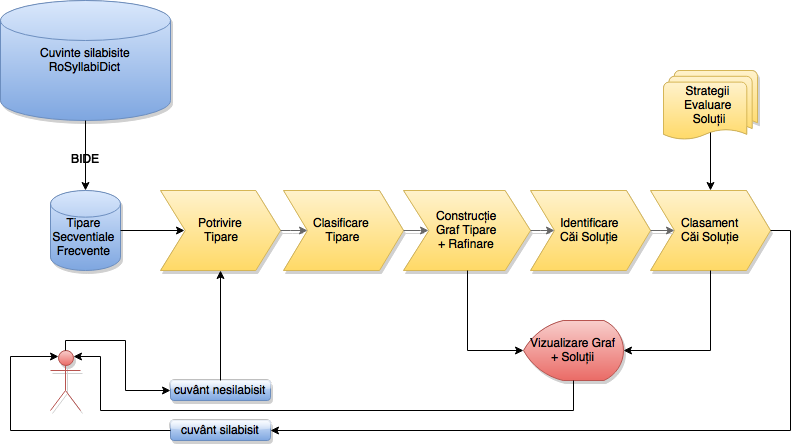
\includegraphics[width=\textwidth]{figures/rosil-flow.png}
    \caption{Diagrama conceptuală a soluției propuse}
    \label{fig:rosil-flow}
\end{figure}

Principalele etape ale metodei sunt următoarele:
\begin{enumerate}
\item Identificarea tiparelor frecvente dintr-un set de cuvinte despărțite în silabe și indexarea acestora.
\item Identificarea tiparelor care prezintă un grad ridicat de potrivire în cadrul cuvântului care se dorește a fi despărțit în silabe
\item Clasificarea acestor tipare în funcție poziția în cuvânt pe care au "potrivit-o" (început, sfârșit, interior).
\item Construirea unui graf cu aceste tipare pe baza potrivirii dintre aceste tipare
\item Eliminarea nodurilor izolate din acest graf
\item Pe baza unor strategii de predicție, se va alege o cale sau mai multe în acest graf, reprezentând soluțiile propuse pentru despărțirea în silabe.
\end{enumerate}

\section{Identificarea tiparelor frecvente}

Pentru a construi setul de tipare frecvente a fost folosită colecția de cuvinte despărțite în silabe în limba română RoSyllabiDict, \cite{bib:BARBU08.495}. Acest set de date conține 525486 de cuvinte despărțite în silabe. 

În vederea analizei setului de date, în cadrul tabelului \ref{table:sdb_counts} se poate observa variația numărului de tipare secvențiale frecvente închise în funcție de valoarea de suport minim.   

\begin{table}[h!]
\centering
\begin{tabular}{|c|c|c|c|c|c|c|c|c|}
\hline
Sup.& Total & Lung. 1 & Lung. 2 & Lung. 3 & Lung. 4 & Lung. 5 & Lung. 6 & Lung. 7\\ 
\hline
\hline
1000 & 648 & 252 & 385 & 11 & 0 & 0 & 0 & 0\\ 
\hline
800 & 890 & 293 & 576 & 21 & 0 & 0 & 0 & 0\\ 
\hline
600 & 1339 & 380 & 903 & 56 & 0 & 0 & 0 & 0\\ 
\hline
400 & 2211 & 523 & 1544 & 143 & 1 & 0 & 0 & 0\\ 
\hline
200 & 4812 & 832 & 3384 & 576 & 20 & 0 & 0 & 0\\ 
\hline
100 & 10461 & 1234 & 6754 & 2309 & 162 & 2 & 0 & 0\\ 
\hline
50 & 22852 & 1824 & 12671 & 7453 & 853 & 47 & 4 & 0\\ 
\hline
20 & 62549 & 2597 & 25731 & 28056 & 5384 & 674 & 90 & 17\\ 
\hline
10 & 129106 & 3271 & 41126 & 63388 & 17812 & 2940 & 454 & 97\\ 
\hline
5 & 256065 & 4146 & 63443 & 123429 & 52271 & 10553 & 1840 & 327\\ 
\hline
2 & 633195 & 5469 & 104254 & 248227 & 186623 & 66915 & 16920 & 3882\\ 
\hline\end{tabular}
\label{table:sdb_counts}
\caption{Numărul de tipare secvențiale frecvente închise pentru setul de date RoSyllabiDict} 
\end{table}

Alegerea unui suport minim cat mai mic asigură prezența a cât mai multor tipare în colecția de tipare folosite ulterior de metodă. Aceasta va creste precizia metodei dar pe de altă parte performanța este influențată de cantitiatea de tipare. 

Cu cât numărul de tipare este mai mare, cautarea de potriviri devine mai lentă, iar pentru a creste performanța, acestea pot fi indexate. În tabelul \ref{table:sdb_patterns} sunt prezentate o serie de tipare frecvente, pentru a le indexa metoda se folosește de o tabela de disperie în care valorile cheilor vor fi reprezentate de silabele concatenate continute de tipare. Un astfel de exemplu se regăseste în cadrul tabelului \ref{table:sdb_index}. 

\begin{table}[h!]
\centering    
\begin{tabular}{|l|l|}    
\hline      
Cheie & Valoare\\
\hline
$a$ 		& $(<a>, 2)$  \\
$libe$ 		& $(<li, be>, 2)$  \\
$programa$ 	& $(<pro, gra, ma>, 2)$  \\
$mare$ 		& $(<ma, re>, 2)$  \\
$mator$ 	& $(<ma, tor>, 2)$  \\
$ti$ 		& $(<ti>, 2)$  \\
$eli$ 		& $(<e, li>, 3)$  \\
$grama$ 	& $(<gra, ma>, 3)$  \\
$sare$ 		& $(<sa, re>, 3)$  \\
$tor$ 		& $(<tor>, 4)$  \\
$li$ 		& $(<li>, 4)$  \\
$e$ 		& $(<e>, 5)$  \\
$ma$ 		& $(<ma>, 5)$  \\
$re$ 		& $(<re>, 6)$  \\
\hline
\end{tabular}
\caption{Exemplu de indexare pentru tipare secvențiale frecvente}
\label{table:sdb_index}               
\end{table}  

Odată având colecția de tipare frecvente indexată, procesul de silabizarea poate fi initial. 
 
\section{Potrivirea tiparelor in vederea silabisirii}

Fie $W$ un cuvânt compus dintr-o secvență de litere, iar $Z_W$ mulțimea tuturor subsecventelor continue ale acestui cuvânt, precum si îndexii de inceput și sfârșit ai acestora.

\begin{ex}
Pentru cuvântul $amator$, tuplele din multimea sunt $Z_{amator}$ sunt ilustrate în cadrul tabelului \ref{table:sdb_substrings}. 
\end{ex}


\begin{table}[b!]
\centering    
\begin{tabular}{|l|l|}    
\hline      
Secventă & Indexi\\
\hline
$a$ 		& $\left[0,1\right), \left[2,3\right)$  \\
$m$ 		& $\left[1,2\right)$  \\
... 		& ...  \\
$amator$ 	& $\left[0,6\right)$  \\

\hline
\end{tabular}
\caption{Mulțimea $Z_{amator}$}
\label{table:sdb_substrings}               
\end{table}  

\begin{defi} Prin \textbf{potrivirea tiparelor} pentru cuvântul $W$, având multimea $Z_W$ asociată, se dorește identificarea tuturor tiparelor frecvente care sunt indexate cu chei care aparțin multimii $Z_W$. Notăm rezultatul acestei operații cu $M_W$. Considerând același cuvânt $amator$, $M_{amator}$ este ilustrată în tabelul \ref{table:sdb_pattern_match}
\end{defi}

\begin{table}[h!]
\centering    
\begin{tabular}{|l|l|}    
\hline      
Tipar frecvent & Indexi potrivire\\
\hline
$(<a>, 2)$			& $\left[0,1\right), \left[2,3\right)$   \\
$(<ma>, 5)$  		& $\left[2,4\right)$\\
$(<ma, tor>, 2)$ 	& $\left[2,6\right)$ \\
$(<tor>, 4)$  		& $\left[4,6\right)$\\
\hline
\end{tabular}
\caption{Exemplu de indexare pentru tipare secvențiale frecvente}
\label{table:sdb_pattern_match}               
\end{table}  

Pentru ca ulterior sa se poată identifica posibile despărțiri în silabe este necesară clasificarea tiparelor frecvente potrivite. Astfel, există patru tipuri de tipare:  

\begin{itemize}
\item tipare de început: ($<a>$,2),
\item tipare intermediare: ($<ma>$,5), ($<a>$,2).
\item tipare de sfarșit: ($<ma, tor>$,2), ($<tor>$,4).  
\item tipare complete (acele tipare frecvente care inglobeaza întreg cuvântul de despărțit).
\end{itemize}

Odată identificate aceste tipare frecvente se pune problema organizării acestora în vederea reconstrucției cuvântului din tipare frecvente. Aceste reconstrucții reprezintă posibile despătiri în silabe. 

Pentru această reconstrucție s-a ales ca structură de date un graf orientat, după cum va fi descris în secțiunea următoare.

\section{Grafuri de tipare}

Odată identificate, tiparele frecvente, trebuie remarcată legătura că în majoritatea cazurilor, există legături între acestea. Prin legături între tipare se întelege ca fie unele se termină în vecinătatea unei litere dintr-un cuvânt, iar altele încep în acea poziție, sau chiar mai mult decat atat, există tipare între care există suprapuneri. 

Pornind de la obervațiile aceastea, în cele ce urmează, va fi arătat că pe baza acestor relatii dintre tiparele frecvente ale unui cuvânt, se vor putea construi lanțuri de tipare secvențiale frecvente, care să reprezinte silibisiri ale cuvântului respectiv.



\section{Strategii de predictie a desparii in silabe} 

\section{Metrici de evaluare}